\documentclass{beamer}
\usepackage{graphicx}
\usepackage{subcaption}
\usepackage{tikz}
\usepackage{pgfplots}

\pgfplotsset{compat=1.18}

\usetheme{Madrid}
\usecolortheme{beaver}
\setbeamertemplate{navigation symbols}{}

\title{Mathematics in Deep Learning}
\author{Lachlan Jones}
\institute{MATH199}
\date{2025}

\begin{document}

\frame{\titlepage}

\begin{frame}
    \frametitle{Mathematics in Deep Learning}
    \begin{figure}
        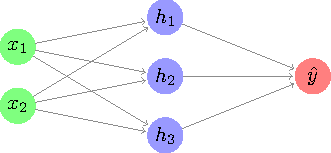
\includegraphics{figures/basic-mlp/main.pdf}
        \caption{MLP network with two inputs and one hidden layer}
    \end{figure}
    \begin{block}{Remark}
        We've tidied up our diagram to not show biases and activation functions, but they're still there and being used in calculations.
    \end{block}
\end{frame}

\begin{frame}
    \frametitle{Mathematics in Deep Learning}
    \begin{minipage}{0.45\textwidth}
        Calculations:
        \[h_{1} = w_{1, 1} \cdot x_1 + w_{1, 2} \cdot x_2 + b_{1}\]
        \[h_{2} = w_{2, 1} \cdot x_1 + w_{2, 2} \cdot x_2 + b_{2}\]
        \[h_{3} = w_{3, 1} \cdot x_1 + w_{3, 2} \cdot x_2 + b_{3}\]
    \end{minipage}
    \hfill
    \begin{minipage}{0.45\textwidth}
        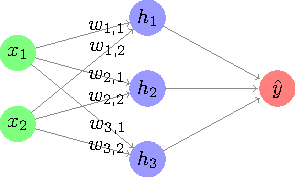
\includegraphics{figures/basic-mlp-weights/main.pdf}
    \end{minipage} \pause
    \vspace{0.5cm}

    This is a typical system of equations, so we can tidy things up with matrix algebra: \pause
    \[
        \begin{bmatrix}
            h_{1} \\
            h_{2} \\
            h_{3}
        \end{bmatrix}
        =
        \begin{bmatrix}
            w_{1, 1} & w_{1, 2} \\
            w_{2, 1} & w_{2, 2} \\
            w_{3, 1} & w_{3, 2} \\
        \end{bmatrix}
        \begin{bmatrix}
            x_1 \\
            x_2
        \end{bmatrix}
        +
        \begin{bmatrix}
            b_1 \\
            b_2 \\
            b_3
        \end{bmatrix}
    \] \pause
    With an activation function, the output of the hidden layer is:
    \[\underline{h} = f(W \cdot \underline{x} + \underline{b})\]
\end{frame}

\begin{frame}
    \frametitle{Mathematics in Deep Learning}
    Typically, architecture is much more complex, with many hidden layers. This is what \alert{deep} learning is referring to.

    \begin{figure}
        \centering
        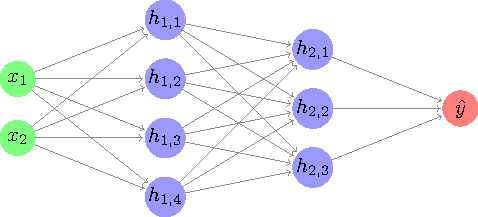
\includegraphics[height=0.5\textheight]{./figures/mlp/main.pdf}
        \caption{Example of what a deep NN could look like}
    \end{figure}
\end{frame}

\begin{frame}
    \frametitle{Mathematics in Deep Learning}
    With all these different edges, deep neural networks have the capacity to learn complex, non-linear relationships between input data (\(\underline{x}\)) and output label (\(\hat{y}\)). \pause
    \vspace{0.5cm}

    Suitable values for these edges need to be determined in a process called training, which uses an algorithm called gradient descent (very similar to \alert{Euler's Method}, i.e. using calculus). 

\end{frame}

\begin{frame}
    \frametitle{Mathematics in Deep Learning}
    Some Examples:
    \begin{itemize}
        \item Using measurements of chemical modifications to human DNA to predict lifetime smoking exposure - this is what my Master's thesis is on \pause
        \item Teaching computers to recognise handwritten digits - \url{https://okdalto.github.io/VisualizeMNIST_web/} \pause
        \item Predicting the most likely word to next appear in a sequence, aka large language models (ChatGPT) \pause
    \end{itemize}

    Each of these use the same connections we saw before, just arranged in different ways to form different \alert{architectures}.
\end{frame}

\end{document}